\documentclass[tikz, border=2pt]{standalone}

\usepackage{amsmath,amssymb}
\usepackage{pgfplots}
\pgfplotsset{compat=1.18}
\usepackage{xcolor}

\definecolor{utnblue}{RGB}{0, 51, 102}
\definecolor{utnred}{RGB}{204, 0, 0}

\begin{document}
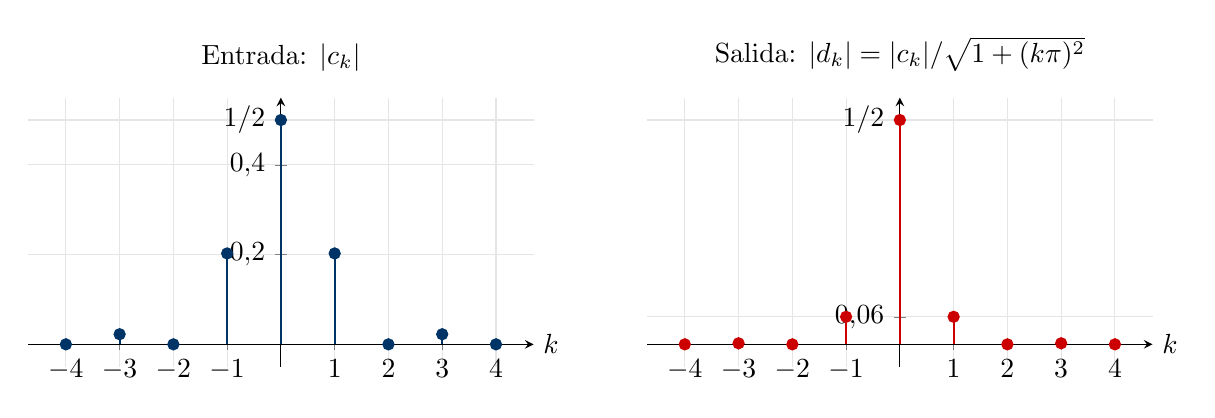
\begin{tikzpicture}

% --- Entrada |c_k| (triángulo) ---
\begin{axis}[
    name=ent,
    width=8cm, height=5cm,
    title={Entrada: $|c_k|$},
    xmin=-4.7, xmax=4.7,
    ymin=-0.05, ymax=0.55,
    xtick={-4,-3,-2,-1,0,1,2,3,4},
    ytick={0, 0.2, 0.4, 0.5},
    yticklabels={$0$, $0{,}2$, $0{,}4$, $1/2$},
    xlabel={$k$},
    axis lines=middle,
    enlargelimits=false,
    grid=major,
    grid style={gray!20},
    every axis x label/.style={at={(ticklabel* cs:1)}, anchor=west},
]
\addplot+[utnblue, thick, ycomb, mark=*, mark options={fill=utnblue, scale=0.9}]
    coordinates {
        (-4, 0) (-3, 0.02252) (-2, 0) (-1, 0.20264) (0, 0.5)
        (1, 0.20264) (2, 0) (3, 0.02252) (4, 0)
    };
\end{axis}

% --- Salida |d_k| ---
\begin{axis}[
    at={(ent.right of east)}, anchor=left of west, xshift=1.0cm,
    width=8cm, height=5cm,
    title={Salida: $|d_k| = |c_k| / \sqrt{1+(k\pi)^2}$},
    xmin=-4.7, xmax=4.7,
    ymin=-0.05, ymax=0.55,
    xtick={-4,-3,-2,-1,0,1,2,3,4},
    ytick={0, 0.0614, 0.5},
    yticklabels={$0$, $0{,}06$, $1/2$},
    xlabel={$k$},
    axis lines=middle,
    enlargelimits=false,
    grid=major,
    grid style={gray!20},
    every axis x label/.style={at={(ticklabel* cs:1)}, anchor=west},
]
\addplot+[utnred, thick, ycomb, mark=*, mark options={fill=utnred, scale=0.9}]
    coordinates {
        (-4, 0) (-3, 0.00237) (-2, 0) (-1, 0.0614) (0, 0.5)
        (1, 0.0614) (2, 0) (3, 0.00237) (4, 0)
    };
\end{axis}

\end{tikzpicture}
\end{document}
